% !Mode:: "TeX:UTF-8"
% !TEX program  = xelatex
\documentclass[a4paper]{article}
\usepackage{amsmath}
\usepackage{amssymb}
\usepackage{ctex}
%\usepackage{braket}
%\usepackage[european]{circuitikz}
\usepackage{multirow}
\usepackage{float}
\usepackage{graphicx}
\usepackage{geometry}
\geometry{left=2.5cm,right=2.5cm,bottom=2.5cm,top=2.5cm}
\title{近代物理实验报告2.2:X荧光分析}
\author{林杨\quad 211840092\quad 物理学院}
\date{2024年5月12日}
\begin{document}
\maketitle
\bibliographystyle{unsrt}
%--------main-body------------

\section{引言}
X荧光分析是一种快速、无损、多元素同时测定的现代技术,已经广泛应用于材料科学、生物医学、地质研究、环境监测、天体物理、文物考古、刑事侦查、工业生产等诸多领域。

\section{实验目的}
\begin{enumerate}
\item 了解能量色散X荧光分析的原理,仪器构成和基本测量、分析方法。
\item 验证Moseley定律,并从实验推出屏蔽常数等。
\item 研究物质对X射线的吸收规律。
\end{enumerate}

\section{实验仪器}
X荧光分析仪、样品。

\section{实验原理}
\subsection{特征X射线}
以一定能量的光子,电子,质子,$\alpha$粒子或其他离子轰击样品,将物质原子中的内壳层电子击出,产生电子空位,原子处于激发态。外壳层电子向内壳层跃迁,填补内壳层电子空位,同时释放出跃迁能量,原子回到基态。跃迁能量以特征X射线形式释放,或能量转移给另一个轨道电子,使该电子发射出来,即俄歇电子发射。另外还可能存在几率较低,主量子数相同,角量子数不同,亚壳层间电子的Coster-Kronig非辐射跃迁。测出特征X射线能谱,即可确定所测样品中元素种类和含量。

当原子中K层电子被击出后,L层或M层的电子填补K层电子空位,同时以一定几率发射特征X射线。L$\to$K产生的X射线叫$K_{\alpha}$系,L层有三个子壳层,允许跃迁使$K_{\alpha}$系有两条谱线$K_{\alpha 1}$和$K_{\alpha 2}$。M$\to$K产生的X射线叫$K_{\beta}$系,M层有五个子壳层,允许跃迁使$K_{\beta}$有$K_{\beta 1}$,$K_{\beta 3}$,$K_{\beta 5}$三条谱线。当原子中L层电子被击出后,M$\to$L跃迁产生的X射线叫L系。图(\ref{Elevel})是特征X射线与电子跃迁能级示意图。
\begin{figure}[H]
\centering
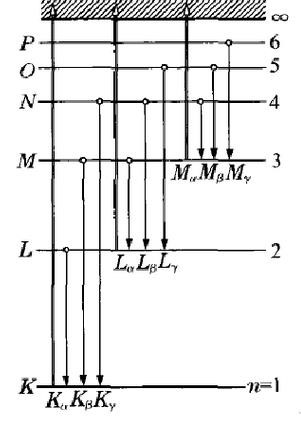
\includegraphics[width=6cm]{fig/Elevel.jpg}\\
\caption{特征X射线系-跃迁能级示意图}\label{Elevel}
\end{figure}
特征X射线的能量为两壳层电子结合能之差,即
\begin{equation}
E_{K_{\alpha}} = B_K - B_L\text{, }E_{K_{\beta}} = B_K - B_M\text{, }E_L = B_L - B_M
\end{equation}
所有元素的K,L系特征X射线能量在几千eV到几十千eV之间。

\subsection{X射线的激发}
X荧光分析中激发X射线的方式一般有三种:
\begin{enumerate}
\item 用质子、$\alpha$粒子或其他离子激发\\
用质子激发特征X射线的分析技术(常记为PIXE)是几种激发方式中分析灵敏度最高的,相对灵敏度达$10^{-6}\sim 10^{-7}$ g/g,绝对灵敏度可达$10^{-9}\sim 10^{-16}$g,而且可以将质子束聚焦、扫描,对样品作微区分析。
\item 用电子激发\\
用电子束激发(常记为EIX),目前主要用在扫描电镜与电子探针中。与PIXE相比,电子激发引起的韧致辐射本底比质子激发大,影响分析灵敏度。一般灵敏度比PIXE低$ 2\sim 3 $个数量级。另外这种激发方式不能在空气中进行,只适用于薄样品。
\item 用X射线或低能$ \gamma $射线激发\\
用X射线或低能$ \gamma $射线激发(记为XIX),常用X光管,放射性同位素作为激发源。这类激发用射线不易聚焦;分析灵敏度亦稍低,相对灵敏度一般为$10^{-5}\sim 10^{-6}$g/g,绝对灵敏度约为$10^{-7}\sim 10^{-8}$g,低于PIXE的灵敏度。
\end{enumerate}

轻便型仪器常用放射性同位素和X光管作激发源。可选用的同位素源主要有$^{55}$Fe,$^{238}$Pu,$^{109}$Cd,$^{241}$Am,$^{57}$Co,$^{153}$Gd等。其中$^{238}$Pu在$\alpha$衰变后发出的$^{234}$U的LX射线,其能量为11.6keV$ \sim $21.7keV,能谱如图(\ref{Pu238})所示。$^{238}$Pu的半衰期为87.7年,用得比较多。
\begin{figure}[H]
	\centering
	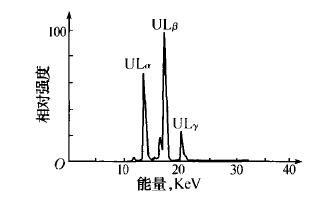
\includegraphics[width=6cm]{fig/Pu238.jpg}\\
	\caption{$^{238}$Pu源的X射线能谱}\label{Pu238}
\end{figure}

\subsection{X射线能谱}
X光管是通过加热阴极K发出的热电子在阴、阳极间高压电场加速下,轰击阳极A(常称阳极靶)产生X射线的。图(\ref{X})是比较典型的X光管(钨靶)产生的X射线谱;它由连续谱和特征谱组成。特征谱决定于靶材,其生成机理如前述。连续谱产生机理如图(\ref{CS})所示。高速电子打入阳极靶,被靶中原子核的库仑场减速,发出韧致辐射。原子核的质量远大于电子质量,此过程中原子核的动能可忽略,因此,韧致辐射发出的光子能量$ h\nu $应等于电子动能的减少,即,
\begin{equation}
h\nu = E_{ki} - E_{kf} = eV - E_{kf}
\end{equation}
\begin{figure}[H]
\centering
\begin{minipage}[!h]{0.48\linewidth}
\begin{center}
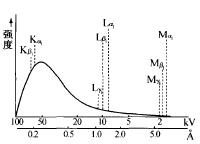
\includegraphics{fig/X.jpg}\\
\caption{X光管激发的X射线谱}\label{X}
\end{center}
\end{minipage}
\begin{minipage}[!h]{0.48\linewidth}
\begin{center}
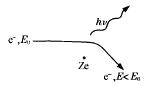
\includegraphics{fig/CS.jpg}\\
\end{center}
\caption{连续谱产生机理示意图}\label{CS}
\end{minipage}
\end{figure}
当电子动能减少到0时,发出的光子能量最大,相应频率最高,波长最短
\begin{equation}
h\nu_0 = eV\text{ , }\lambda_0 V = \frac{hc}{e}
\end{equation}
由上式可知,连续谱有与加速高压成反比的短波限$\lambda_0$,它与靶材和光管电流均无关。测出短波限,也可以推算出普朗克常数$ h $。在频率不太高时,连续谱的强度近似为
$I(\nu)=\text{常数}\cdot Z(\nu_0-\nu)$,辐射的空间分布像偶极振子的辐射分布。频率高时偏前向。

连续谱的强度分布与X光管阳极与阴极间电压$ V $,光管电流$ i $和靶元素的原子序数$ Z $有关,其关系为$I\propto ZiV^2$,连续谱最大强度对应的波长$\lambda_{I_{max}}$约为短波限$\lambda_0$的1.5倍($\lambda_{I_{max}}\approx 1.5\lambda_0$)。

特征X射线强度,当X光管靶材一定后,与管电压$ V $和管电流$ i $的关系为$ I \propto (V-V_0)^n i  $,其中$V_0$为激发电势,它对应于激发某线系所需的最低能量。当$ V $是$V_0$的$ 2\sim 3 $倍时,$ n\approx 2 $,当$V > 3V_0$时,$n\approx 1$。

\paragraph{XIX能谱特征}~\\
XIX技术中,人射光子除与样品中原子发生光电作用产生内壳层空位外,还可以发生相干散射和非相干散射(康普顿散射),这些散射光子进入探测器,形成XIX分析中的散射本底。另外,样品中激发出的光电子又会产生轫致辐射,但这产生的本底比散射光子本底小得多,且巨能量也较低,一般在3keV以下。所以XIX能谱特征是:特征X射线峰叠加在散射光子峰之间的平坦的连续本底谱上。如图(\ref{5})能谱示意图所示。a峰是相干散射光子峰,b是康普顿散射光子峰,c是特征X射线峰,d是散射光子在探测器中的康普顿边缘。
\begin{figure}[H]
\centering
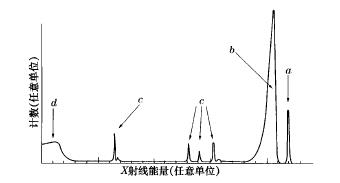
\includegraphics[width=12cm]{fig/5.jpg}\\
\caption{光子激发的特征X射线能谱示意图}\label{5}
\end{figure}
测量特征X射线常用Si(Li)探测器,它的能量分辨率高,适用于多元素同时分析,也可选用Ge(Li)或高纯Ge探测器,但均价格昂贵。另外还有电致冷Si-PIN ,CdTe,HgIz等探测器在某些特定仪器中使用。

\subsection{X荧光分析}
在X荧光分析中,对于轻元素(一般指Z<45的元素)通常测其KX射线,对于重元素($ Z>45 $的元素),因其KX射线能量较高且比LX射线强度弱,常测其LX射线,这样测量的特征X射线能量一般在20keV以下。正比计数管在此能量范围,探测效率较高,其能量分辨率虽比Si(Li)探测器差,但远好于NaI(Tl)闪烁探测器,质量好的正比管5.89keV处分辨率优于14\%,能满足一般实验的需要。

用正比计数管作探测器的X荧光分析系统如图(\ref{XIXdevice})所示。为防止探测系统中脉冲叠加,除适当选择放射源强度外,前置放大器和主放大器要有抗堆积措施。多道分析器适宜作多元素同时分析,数据可由计算机获取和处理。
\begin{figure}[H]
\centering
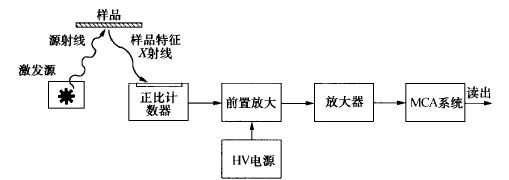
\includegraphics[width=12cm]{fig/6.jpg}\\
\caption{XIX装置示意图}\label{XIXdevice}
\end{figure}

\section{实验内容}
\begin{enumerate}
\item X荧光分析仪的能量、效率刻度
仪器在实测样品前需要作能量和效率标定。常用的方法有两种:
\begin{enumerate}
\item 用标准X射线源进行校刻\\
即用一组射线能量和强度已知的源,探测器对其张一固定立体角,在固定时间内测出对应能量的X射线峰和计数,作出能量效率校正曲线。常用的校刻标准源及其$K_{\alpha}$ X射线能量是$^{54}$Mn(5.41keV)、$^{55}$Fe(5.90keV)、$^{57}$Co(6.4keV)、$^{65}$Zn(8.05keV)、$^{85}$Sr(13.39)、$^{88}$Y(14.16)keV、$^{57}$Co(14.4keV)。
\item 用标准样品进行校刻。可以选一组特征X射线峰相隔较远,峰不重叠的元素,以不同的相对含量制成一组样品,在与测试样品相同的几何条件下,测出各元素的特征X射线峰所在的道址和相应的计数。由特征X射线能量数据表查出标样中各元素特征X射线的能量,作出能量一道址曲线和相对含量—特征峰强度曲线。
\end{enumerate}
本实验采用的是方法二。
\end{enumerate}

\section{实验数据}
\begin{enumerate}
\item 已知材料的X荧光特征能谱和道址\\
\begin{table}[htbp]
	\begin{tabular}{|c|cc|cc|cc|c|c|c|}
	\hline
	样品      & \multicolumn{2}{c|}{$Y_{2}O_{3}$}              & \multicolumn{2}{c|}{Fe-Zn合金}             & \multicolumn{2}{c|}{Ta}              & Ti      & Mo       & Cu      \\ \hline
	道数      & \multicolumn{1}{c|}{1135}    & 1282    & \multicolumn{1}{c|}{480}     & 656     & \multicolumn{1}{c|}{619}    & 711    & 336     & 1325     & 612     \\ \hline
	能量/keV & \multicolumn{1}{c|}{14.9584} & 16.7378 & \multicolumn{1}{c|}{6.40384} & 8.03886 & \multicolumn{1}{c|}{8.1461} & 9.3431 & 4.51084 & 17.47934 & 8.04778 \\ \hline
	线系      & \multicolumn{1}{c|}{$K_\alpha$}      & {$K_\beta$}     & \multicolumn{1}{c|}{$K_\alpha$}    & {$K_\alpha$}      & \multicolumn{1}{c|}{$L_\alpha$}     & {$L_\beta$}      & {$K_\alpha$}      & {$K_\alpha$}       & {$K_\alpha$}      \\ \hline
\end{tabular}
\end{table}

\item 能量-道址曲线\\
画出道址(Channel)与能量(Energy)的散点图,并进行线性拟合,如图(\ref{E-Channel}):
\begin{figure}[!h]
\centering
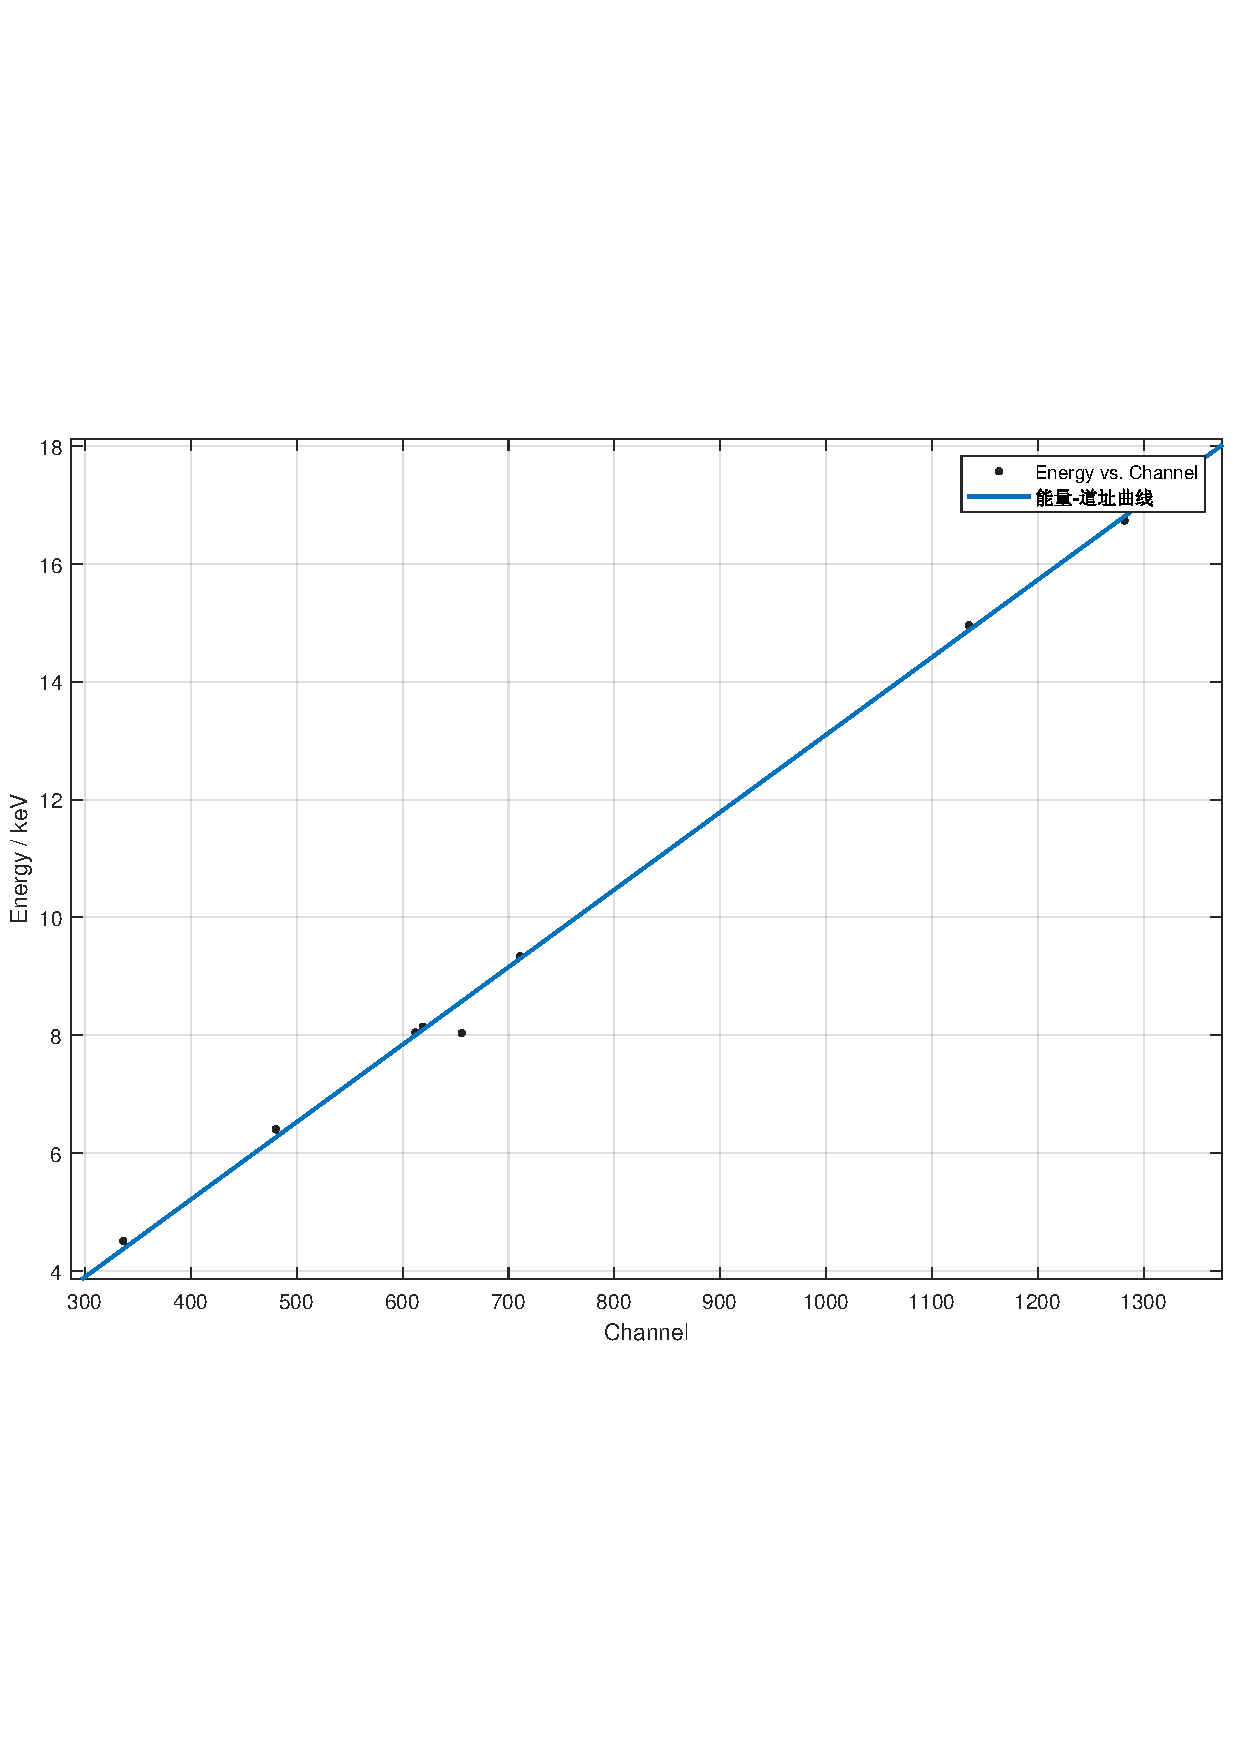
\includegraphics[width=12cm]{fig/E_C.pdf}\\
\caption{能量-道址曲线}\label{E-Channel}
\end{figure}
从图中可以看出,拟合曲线的相关系数为$R^2 = 0.9980$,说明数据的线性非常好,给出能量与道址的关系式:
\begin{equation}
E = 0.0131*Channel-0.0421 \text{keV}\label{E-Channel_Eqn}
\end{equation}

\item 测量未知材料样品\\
我们选择了一些未知材料,测量其化学组成(不包含组成含量)
\begin{table}[]
	\begin{tabular}{|c|cc|cc|cc|cc|}
	\hline
	测量物质                     & \multicolumn{2}{c|}{未知石块}               & \multicolumn{2}{c|}{灰色高级仪器架}       & \multicolumn{2}{c|}{扁扁的黑色柱块}     & \multicolumn{2}{c|}{五元纸币}       \\ \hline
	道数                       & \multicolumn{1}{c|}{481} & 1112-1614 & \multicolumn{1}{c|}{653} & 478 & \multicolumn{1}{c|}{477} & 1082 & \multicolumn{1}{c|}{146} & 337                    \\ \hline
	能量/keV                       & \multicolumn{1}{c|}{6.2951}    & 14.5342-20.6723             & \multicolumn{1}{c|}{7.8963}    &  6.2318   & \multicolumn{1}{c|}{6.2187}    & 14.1042     & \multicolumn{1}{c|}{1.6355}    &  4.1397   \\ \hline
	可能元素                     & \multicolumn{1}{c|}{Fe}  & 40-48号元素     & \multicolumn{1}{c|}{Cu}    & Fe  & \multicolumn{1}{c|}{Fe}  & Sr  & \multicolumn{1}{c|}{Si或者Rb?}    & Sc?  \\ \hline
	\multicolumn{1}{|l|}{结论} & \multicolumn{2}{c|}{可能是铁矿石}          & \multicolumn{2}{c|}{可能是铁架子}          & \multicolumn{2}{c|}{可能是掺有锶的铁块}           & \multicolumn{2}{c|}{}          \\ \hline
	\multicolumn{1}{|l|}{测量人}   & \multicolumn{2}{c|}{赵羽竹}                & \multicolumn{2}{c|}{杨照}        & \multicolumn{2}{c|}{林杨}         & \multicolumn{2}{c|}{拓展}  \\ \hline
\end{tabular}
\end{table}
\end{enumerate}

\section{思考题}
\subsection{测量样品与标准样品计数率相差很大,对测量有何影响?}
没有太大的影响。测量样品与标准样品在计数率上的差别来自于化学组成占比上的不同。只要正确辨认出道址与元素的对应关系,进而确定道址与能量的对应关系,就可以忽略在计数率上的差别。
\subsection{液体样品可以用X荧光分析测其成分吗?用何方法,要注意什么?}
可以。要注意盛放液体样品的溶液,溶液应对X射线有良好的透过性。或者采用对照试验,在实验组中去除对照组的能谱。

\nocite{jiaocai}
\bibliography{ref}
\end{document}